\documentclass[a4paper, 12pt]{article}%тип документа

\usepackage[14pt]{extsizes} % для того чтобы задать нестандартный 14-ый размер шрифта

%отступы
\usepackage[left=2cm,right=2cm,top=2cm,bottom=3cm,bindingoffset=0cm]{geometry}

%Русский язык
\usepackage[T2A]{fontenc} %кодировка
\usepackage[utf8]{inputenc} %кодировка исходного кода
\usepackage[english,russian]{babel} %локализация и переносы

%Вставка картинок
\usepackage{wrapfig}
\usepackage{graphicx}
\graphicspath{{pictures/}}
\DeclareGraphicsExtensions{.pdf,.png,.jpg}

%Графики
\usepackage{multirow}
\usepackage{pgfplots}
\pgfplotsset{compat=1.9}

%Математика
\usepackage{amsmath, amsfonts, amssymb, amsthm, mathtools}

%Заголовок
\author{Валеев Рауф Раушанович \\
группа 825}
\title{\textbf{Работа 2.3.1 \\ 
Современные методы измерения и получения вакуума}}
\begin{document}
\maketitle
\section*{Краткая теоритическая справка}
\subsection*{Основные понятия}
Основы процесса откачки и связанные с ним понятия рассмотрим на примере простейшей вакуумной системы (рис. 1).

\begin{figure}[h]
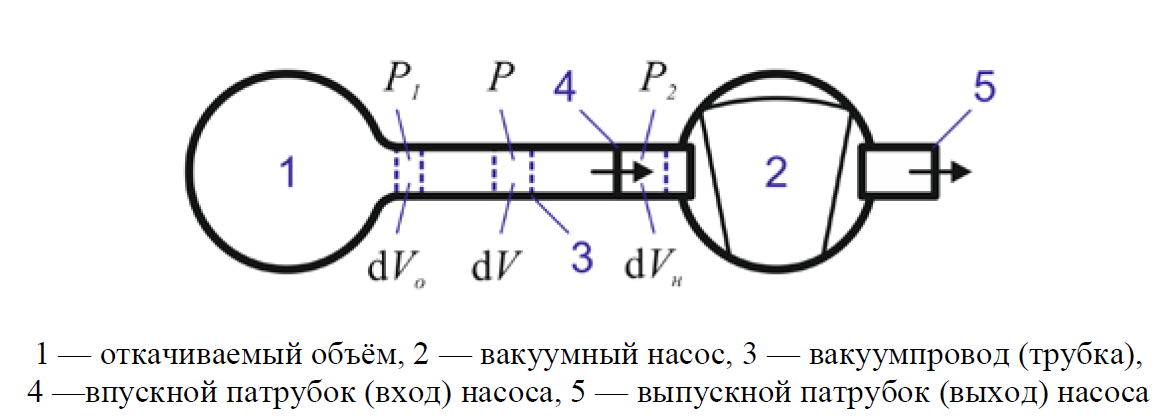
\includegraphics[width = \textwidth]{231_3.png}
\caption{Простейшая вакуумная система}
\end{figure}
Здесь и далее $L$ - единица измерения длины, $M$ - единица измерения массы, $T$ - единица измерения времени.
\begin{enumerate}
\item \textbf{Предельное остаточное давление} (предельный вакуум) $P_{\text{пр}} [L^{-1}MT^{-2}]$ - наименьшее давление газа, которое формируется в процессе откачки в рассматриваемом сечении вакуумпровода (рассматриваемой точке вакуумной системы). Обычно выделяют предельное давление в камере или на входе в насос.
\item \textbf{Наибольшее выпускное давление} $[L^{-1}MT^{-2}]$ - максимально допустимое давление газа на входе насоса.
\item \textbf{Быстрота откачивающего действия} (скорость откачки) вакуумной системы $S [L^3T^{-1}]$ - объем газа, проходящий через рассматриваемое сечение вакуумпровода в единицу времени при текущем давлении в данном сечении:
\[S = \dfrac{dV}{dT}\]
Следовательно быстродействие насоса $S_{\text{н}}$ определяется как:
\[ S_{ \text{н} } = \dfrac{dV_{ \text{н} }}{ dt } \]
А эффективная скорость откачки камеры $S_0$:
\[S_0 = \dfrac{ dV_0 }{ dt } \]
\item Падение давления вдоль вакуумпровода $ \Delta P = P_1 - P_2 $ определяется его \textbf{пропускной способностью} (проводимостью) $ U [L^3 T^{-1} ] $:
\[ U = \dfrac{Q}{P_1 - P_2} \]
где $Q [L^2 M T^{-3}]$ - \textbf{поток газа} через вакуумпровод с соответствующими давлениями на концах.
\item Величина $Z [L^{-3}T]$, обратная проводимости, называется импедансом вакуумпровода:
\[Z=\dfrac{1}{U}\]
В общем случае указанные величины $S$, $U$, $Q$, $Z$ как и сами давления $P_1$ и $P_2$ зависят от времени. Но в конце процесса откачки устанавливается квазистационарный режим, при котором поток газа становится практически постоянным и равным количеству поступающего в систему газа в единицу времени вследствие наличия течей, т.е. нарушения герметичности (в основном в местах механического соединения отдельных узлов вакуумной системы). Для стационарного режима можно записать условие непрерывности потока откачиваемого газа:
\[P_1 S_0 = PS = P_2 S_{\text{н}} = Q \]
\item \textbf{Основное уравнение вакуумной техники}
\[\dfrac{1}{S_0} = \dfrac{1}{S_{ \text{н} }} + \dfrac{1}{U}\]
\end{enumerate}
\subsection*{Проводимость длинного трубопровода}
\[U_{\text{тр}} = \dfrac{Q}{P_2 - P_1} = P\dfrac{\pi R^4}{8 \nu L} \sim \dfrac{R^4}{L} \dfrac{P}{\sqrt{Tm}}\]
\[U_{\text{тр}} = \dfrac{Q}{P_2 - P_1} = \dfrac{4}{3} \dfrac{R^3}{L}\sqrt{\dfrac{2 \pi k T}{m}} \sim \dfrac{R^3}{L} \sqrt{\dfrac{T}{m}} \]
В случае последовательного соединения:
\[U_{\Sigma} = \dfrac{1}{Z_{\Sigma}} = \dfrac{1}{\Sigma Z_i}\]

\[S_0 = \dfrac{S_{\text{н}}U_{\Sigma}}{S_{\text{н}} + U_{\Sigma}} = \dfrac{S_{\text{н}}}{\dfrac{S_{\text{н}}}{U_{\Sigma}} + 1} \approx S_{\text{н}} \]	
\subsection*{Время откачки}
Положим, что за промежуток $dt$ давление в откачиваемом объеме $V_0$ снижается на $dP_1$. Тогда за промежуток времени $dt$ количество газа, поступающего в трубу равно $S_0 P_1 dt$, а эта же убыль газа в объеме равна $V_0 dP_1$, следовательно 
\[S_0 P_1 dt = -V_0 dP_1\]
\[dt = -\dfrac{V_0}{S_0} \dfrac{dP_1}{P_1}\]
\[dt = -V_0 \left( \dfrac{1}{S_{ \text{н} }} + \dfrac{1}{U} \right) \dfrac{dP_1}{P_1}\]
Итого получаем, что 
\[P(t) = P_1 \exp \left( -\dfrac{S_0}{V_0} t \right) \] 
\section*{Экспериментальная установка}
\begin{figure}[h]
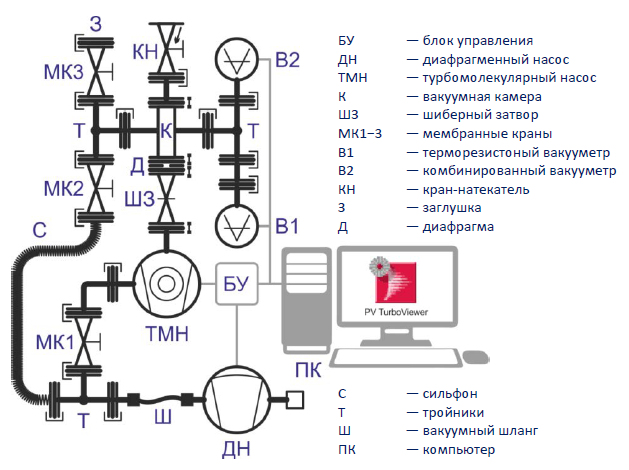
\includegraphics[width = \textwidth]{231_1.png}
\caption{Схема экпериментальной установки}
\end{figure}

Экспериментальный стенд выполнен на основе компактного безмасляного высоковакуумного откачного поста Pfeiffer Vacuum серии HiCube 80 Eco с диафрагменным и турбомолекулярным насосами, вакуумметров Pfeiffer Vacuum серии DigiLine, и вакуумных быстроразъёмных компонентов. Управление основными функциями откачного поста, контроль и запись параметров установки осуществляется блоком управления (БУ) через цифровой интерфейс RS-485 с помощью специального программного обеспечения PV TurboViewer8.
Вакуумный пост Pfeiffer Vacuum HiCube 80 Eco (PM S03 555 А) выполнен на базе диафрагменного форвакуумного насоса MVP 015 (ДН) и турбомолекулярного насоса HiPace 80 (ТМН). Откачка вакуумной камеры (К) может происходить как двумя насосами (ТМН и ДН) через шиберный затвор (ШЗ) и мембранный кран 1 (МК1), так и только форвакуумным насосом (ДН) по схеме «байпас» (англ. bypass — обходной путь), выполненной на основе вакуумных компонентов: сильфона (С), мембранного крана 2 (МК2), тройников (Т), переходников, шланга (Ш). Для контроля и измерения давления в вакуумной камере используются цифровой вакууметр PPT 100 (В1) типа Пирани (терморезисторный) и комбинированный вакуумметр MPT 100 (В2) типов Пирани (терморезисторный) и холодный катод (инвертированный магнетрон). Контролированный напуск воздушной атмосферы в камеру осуществляется через кран-натекатель EVN 116 (КН) с регулируемым потоком. Дополнительный выход с краном 3 (МК3) закрыт заглушкой (З) и служит для присоединения дополнительного объёма в случае необходимости.

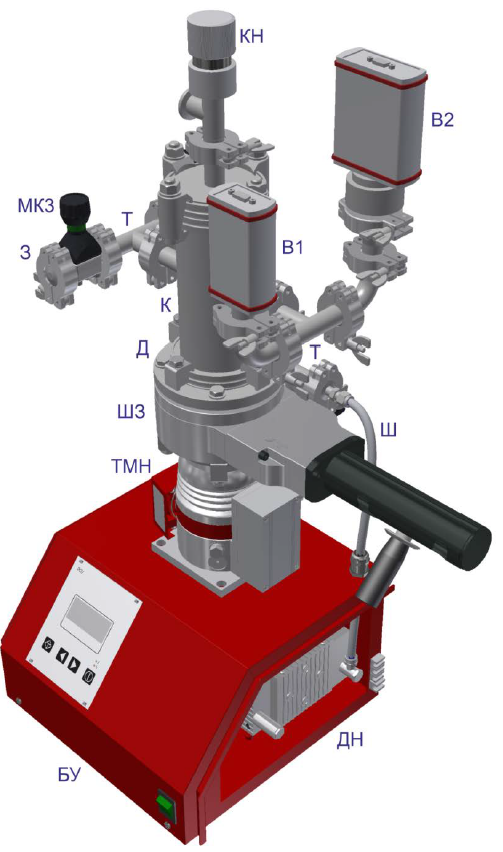
\includegraphics[width = 0.8\textwidth]{231_2.png}

\section*{Ход работы}
\subsection*{Подготовка оборудования}
\begin{enumerate}
\item В первую очередь нужно выровнять давление во всех частях установки.
\item Затем впускаем атмосферный воздух в установку через кран-натекатель с верхней и нижней ручкой регулировки.
\item Далее нужно отгорадить систему от внешней атмосферы, чтобы создать вакуум.
\item Готовим компьютер и блок управления установкой к работе и записи данных.
\end{enumerate}
\subsection*{Определение откачиваемого объёма и измерение скорости откачки форвакуумным насосом}
\begin{enumerate}
\item Выключаем турбомолекулярный насос.
\item Откачиваем установку форвакуумным насосом.
\item Присоединяем к установке сильфон с воздухом при атмосферном давлении. ($V_{\text{сильфона}} = V_0 = 265 ml$).
\item Выравниваем давление в сильфоне и вакуумной камере экспериментального стенда.
\item Выравниваем давление в вакуумной камере К и форвакуумной магистрали установки.
\item Напустим воздух в установку до атмосферного давления.
\item Готовим установку к повтору предыдущих пунктов. Повторяем их еще 1-2 раза.
\item По данным, полученным с установки считаем все объемы.
$P_{\text{для камеры}} = 220 mbar$, $P_{\text{для всей установки}} = 170 mbar \Rightarrow V_{\text{камеры}} = \dfrac{P_{\text{атм}} V_0}{P_1} - V_{0} \approx (0,84 \pm 0,05)$ л,  $V{\text{всей установки}} = \dfrac{P_{\text{атм}} V_0}{P_2} \approx (1,26 \pm 0,05) $ л, $ \Rightarrow$  \\ 
$V{\text{форвакуумной магистрали}} = (0,5 \pm 0,05) $ л

\begin{tabular}{|c|c|c||ccc}
\hline
\multicolumn{3}{|c|}{1} & \multicolumn{3}{c|}{2} \\ \hline
$t, c$ & $P, mbar$ & $\sigma_P, mbar$ & \multicolumn{1}{c|}{$t, c$} & \multicolumn{1}{c|}{$P, mbar$} & \multicolumn{1}{c|}{$\sigma_P, mbar$} \\ \hline
2 & 700,0 & 0,1 & \multicolumn{1}{c|}{2} & \multicolumn{1}{c|}{1000,0} & \multicolumn{1}{c|}{0,1} \\ \hline
4 & 560,0 & 0,1 & \multicolumn{1}{c|}{4} & \multicolumn{1}{c|}{480,0} & \multicolumn{1}{c|}{0,1} \\ \hline
6 & 400,0 & 0,1 & \multicolumn{1}{c|}{6} & \multicolumn{1}{c|}{340,0} & \multicolumn{1}{c|}{0,1} \\ \hline
8 & 320,0 & 0,1 & \multicolumn{1}{c|}{8} & \multicolumn{1}{c|}{220,0} & \multicolumn{1}{c|}{0,1} \\ \hline
10 & 300,0 & 0,1 & \multicolumn{1}{c|}{10} & \multicolumn{1}{c|}{160,0} & \multicolumn{1}{c|}{0,1} \\ \hline
12 & 300,0 & 0,1 & \multicolumn{1}{c|}{12} & \multicolumn{1}{c|}{120,0} & \multicolumn{1}{c|}{0,1} \\ \hline
14 & 300,0 & 0,1 & \multicolumn{1}{c|}{14} & \multicolumn{1}{c|}{90,0} & \multicolumn{1}{c|}{0,1} \\ \hline
16 & 300,0 & 0,1 & \multicolumn{1}{c|}{16} & \multicolumn{1}{c|}{68,0} & \multicolumn{1}{c|}{0,1} \\ \hline
18 & 300,0 & 0,1 & \multicolumn{1}{c|}{18} & \multicolumn{1}{c|}{58,0} & \multicolumn{1}{c|}{0,1} \\ \hline
20 & 230,0 & 0,1 & \multicolumn{1}{c|}{20} & \multicolumn{1}{c|}{44,0} & \multicolumn{1}{c|}{0,1} \\ \hline
22 & 180,0 & 0,1 & \multicolumn{1}{c|}{22} & \multicolumn{1}{c|}{37,0} & \multicolumn{1}{c|}{0,1} \\ \hline
24 & 150,0 & 0,1 & \multicolumn{1}{c|}{24} & \multicolumn{1}{c|}{31,0} & \multicolumn{1}{c|}{0,1} \\ \hline
26 & 120,0 & 0,1 & \multicolumn{1}{c|}{26} & \multicolumn{1}{c|}{26,0} & \multicolumn{1}{c|}{0,1} \\ \hline
28 & 98,0 & 0,1 & \multicolumn{1}{c|}{28} & \multicolumn{1}{c|}{20,0} & \multicolumn{1}{c|}{0,1} \\ \hline
30 & 83,0 & 0,1 & \multicolumn{1}{c|}{30} & \multicolumn{1}{c|}{18,0} & \multicolumn{1}{c|}{0,1} \\ \hline
32 & 69,0 & 0,1 & \multicolumn{1}{c|}{32} & \multicolumn{1}{c|}{15,0} & \multicolumn{1}{c|}{0,1} \\ \hline
34 & 62,0 & 0,1 & \multicolumn{1}{c|}{34} & \multicolumn{1}{c|}{13,0} & \multicolumn{1}{c|}{0,1} \\ \hline
36 & 55,0 & 0,1 & \multicolumn{1}{c|}{36} & \multicolumn{1}{c|}{11,0} & \multicolumn{1}{c|}{0,1} \\ \hline
38 & 46,0 & 0,1 & \multicolumn{1}{c|}{38} & \multicolumn{1}{c|}{9,5} & \multicolumn{1}{c|}{0,1} \\ \hline
40 & 38,0 & 0,1 & \multicolumn{1}{c|}{40} & \multicolumn{1}{c|}{8,5} & \multicolumn{1}{c|}{0,1} \\ \hline
42 & 35,0 & 0,1 & \multicolumn{1}{c|}{42} & \multicolumn{1}{c|}{7,5} & \multicolumn{1}{c|}{0,1} \\ \hline
44 & 32,0 & 0,1 & \multicolumn{1}{c|}{44} & \multicolumn{1}{c|}{6,8} & \multicolumn{1}{c|}{0,1} \\ \hline
46 & 29,0 & 0,1 & \multicolumn{1}{c|}{46} & \multicolumn{1}{c|}{6,4} & \multicolumn{1}{c|}{0,1} \\ \hline
48 & 25,0 & 0,1 & \multicolumn{1}{c|}{48} & \multicolumn{1}{c|}{6,1} & \multicolumn{1}{c|}{0,1} \\ \hline
50 & 21,0 & 0,1 & \multicolumn{1}{c|}{50} & \multicolumn{1}{c|}{5,7} & \multicolumn{1}{c|}{0,1} \\ \hline
52 & 18,0 & 0,1 & \multicolumn{1}{c|}{52} & \multicolumn{1}{c|}{5,4} & \multicolumn{1}{c|}{0,1} \\ \hline
54 & 17,0 & 0,1 & \multicolumn{1}{c|}{54} & \multicolumn{1}{c|}{5,1} & \multicolumn{1}{c|}{0,1} \\ \hline
56 & 16,0 & 0,1 & \multicolumn{1}{c|}{56} & \multicolumn{1}{c|}{4,9} & \multicolumn{1}{c|}{0,1} \\ \hline
58 & 14,0 & 0,1 & \multicolumn{1}{c|}{58} & \multicolumn{1}{c|}{4,6} & \multicolumn{1}{c|}{0,1} \\ \hline
60 & 13,0 & 0,1 & \multicolumn{1}{c|}{60} & \multicolumn{1}{c|}{4,4} & \multicolumn{1}{c|}{0,1} \\ \hline
62 & 11,0 & 0,1 & \multicolumn{1}{c|}{62} & \multicolumn{1}{c|}{4,1} & \multicolumn{1}{c|}{0,1} \\ \hline
64 & 10,0 & 0,1 & \multicolumn{1}{c|}{64} & \multicolumn{1}{c|}{3,9} & \multicolumn{1}{c|}{0,1} \\ \hline
66 & 9,3 & 0,1 & \multicolumn{1}{c|}{66} & \multicolumn{1}{c|}{3,9} & \multicolumn{1}{c|}{0,1} \\ \hline
68 & 8,7 & 0,1 & \multicolumn{1}{c|}{68} & \multicolumn{1}{c|}{3,8} & \multicolumn{1}{c|}{0,1} \\ \hline
70 & 8,1 & 0,1 & \multicolumn{1}{c|}{70} & \multicolumn{1}{c|}{3,7} & \multicolumn{1}{c|}{0,1} \\ \hline
72 & 7,7 & 0,1 & \multicolumn{1}{c|}{72} & \multicolumn{1}{c|}{3,6} & \multicolumn{1}{c|}{0,1} \\ \hline
74 & 7,1 & 0,1 & \multicolumn{1}{c|}{74} & \multicolumn{1}{c|}{3,6} & \multicolumn{1}{c|}{0,1} \\ \hline
\end{tabular}

\begin{tabular}{|c|c|c||ccc}
\hline
\multicolumn{3}{|c|}{1} & \multicolumn{3}{c|}{2} \\ \hline
$t, c$ & $P, mbar$ & $\sigma_P, mbar$ & \multicolumn{1}{c|}{$t, c$} & \multicolumn{1}{c|}{$P, mbar$} & \multicolumn{1}{c|}{$\sigma_P, mbar$} \\ \hline
76 & 6,8 & 0,1 & \multicolumn{1}{c|}{76} & \multicolumn{1}{c|}{3,5} & \multicolumn{1}{c|}{0,1} \\ \hline
78 & 6,5 & 0,1 & \multicolumn{1}{c|}{78} & \multicolumn{1}{c|}{3,5} & \multicolumn{1}{c|}{0,1} \\ \hline
80 & 6,3 & 0,1 & \multicolumn{1}{c|}{80} & \multicolumn{1}{c|}{3,4} & \multicolumn{1}{c|}{0,1} \\ \hline
82 & 6,1 & 0,1 & \multicolumn{1}{c|}{82} & \multicolumn{1}{c|}{3,4} & \multicolumn{1}{c|}{0,1} \\ \hline
84 & 5,9 & 0,1 & \multicolumn{1}{c|}{84} & \multicolumn{1}{c|}{3,3} & \multicolumn{1}{c|}{0,1} \\ \hline
86 & 5,7 & 0,1 & \multicolumn{1}{c|}{86} & \multicolumn{1}{c|}{3,3} & \multicolumn{1}{c|}{0,1} \\ \hline
88 & 5,5 & 0,1 & \multicolumn{1}{c|}{88} & \multicolumn{1}{c|}{3,3} & \multicolumn{1}{c|}{0,1} \\ \hline
90 & 5,4 & 0,1 & \multicolumn{1}{c|}{90} & \multicolumn{1}{c|}{3,2} & \multicolumn{1}{c|}{0,1} \\ \hline
92 & 5,2 & 0,1 & \multicolumn{1}{c|}{92} & \multicolumn{1}{c|}{3,2} & \multicolumn{1}{c|}{0,1} \\ \hline
94 & 5,0 & 0,1 & \multicolumn{1}{c|}{94} & \multicolumn{1}{c|}{3,2} & \multicolumn{1}{c|}{0,1} \\ \hline
96 & 4,9 & 0,1 & \multicolumn{1}{c|}{96} & \multicolumn{1}{c|}{3,1} & \multicolumn{1}{c|}{0,1} \\ \hline
98 & 4,8 & 0,1 & \multicolumn{1}{c|}{98} & \multicolumn{1}{c|}{3,1} & \multicolumn{1}{c|}{0,1} \\ \hline
100 & 4,6 & 0,1 & \multicolumn{1}{c|}{100} & \multicolumn{1}{c|}{3,1} & \multicolumn{1}{c|}{0,1} \\ \hline
102 & 4,5 & 0,1 & \multicolumn{1}{c|}{102} & \multicolumn{1}{c|}{3,1} & \multicolumn{1}{c|}{0,1} \\ \hline
104 & 4,4 & 0,1 & \multicolumn{1}{c|}{104} & \multicolumn{1}{c|}{3,1} & \multicolumn{1}{c|}{0,1} \\ \hline
106 & 4,2 & 0,1 & \multicolumn{1}{c|}{106} & \multicolumn{1}{c|}{3,0} & \multicolumn{1}{c|}{0,1} \\ \hline
108 & 4,1 & 0,1 & \multicolumn{1}{c|}{108} & \multicolumn{1}{c|}{3,0} & \multicolumn{1}{c|}{0,1} \\ \hline
110 & 4,1 & 0,1 & \multicolumn{1}{c|}{110} & \multicolumn{1}{c|}{3,0} & \multicolumn{1}{c|}{0,1} \\ \hline
112 & 3,9 & 0,1 & \multicolumn{1}{c|}{112} & \multicolumn{1}{c|}{3,0} & \multicolumn{1}{c|}{0,1} \\ \hline
114 & 3,9 & 0,1 & \multicolumn{1}{c|}{114} & \multicolumn{1}{c|}{3,0} & \multicolumn{1}{c|}{0,1} \\ \hline
116 & 3,9 & 0,1 & \multicolumn{1}{c|}{116} & \multicolumn{1}{c|}{2,9} & \multicolumn{1}{c|}{0,1} \\ \hline
118 & 3,8 & 0,1 &  &  &  \\ \cline{1-3}
120 & 3,8 & 0,1 &  &  &  \\ \cline{1-3}
122 & 3,8 & 0,1 &  &  &  \\ \cline{1-3}
124 & 3,7 & 0,1 &  &  &  \\ \cline{1-3}
126 & 3,7 & 0,1 &  &  &  \\ \cline{1-3}
128 & 3,7 & 0,1 &  &  &  \\ \cline{1-3}
130 & 3,7 & 0,1 &  &  &  \\ \cline{1-3}
132 & 3,6 & 0,1 &  &  &  \\ \cline{1-3}
134 & 3,6 & 0,1 &  &  &  \\ \cline{1-3}
136 & 3,6 & 0,1 &  &  &  \\ \cline{1-3}
138 & 3,6 & 0,1 &  &  &  \\ \cline{1-3}
140 & 3,6 & 0,1 &  &  &  \\ \cline{1-3}
142 & 3,5 & 0,1 &  &  &  \\ \cline{1-3}
144 & 3,5 & 0,1 &  &  &  \\ \cline{1-3}
146 & 3,5 & 0,1 &  &  &  \\ \cline{1-3}
148 & 3,5 & 0,1 &  &  &  \\ \cline{1-3}
150 & 3,5 & 0,1 &  &  &  \\ \cline{1-3}
152 & 3,5 & 0,1 &  &  &  \\ \cline{1-3}
\end{tabular}
\newpage
\item считаем эффективную скорость форвакуумной откачки, для этого мы в на графике $ln(P/P_1)$ от $t$ ищем наклон графика на интервале $10-100$ мбар. Потом считаем $\tau = - \dfrac{t}{ln(P/P_1)} = (16,06 \pm 0,02)$ с.
А далее, зная объем камеры расчитываем эффективную скорость откачки $S_0 = V{\text{всей установки}} / \tau \approx (0,25 \pm 0,05) m^3/c$
\item Зная $S_0$ и $S_{\text{н}}$ мы находим $U$ по формуле 
\[U = \dfrac{S_{\text{н}} - S_0}{S_{\text{н}} \cdot S_0} \approx 0,2 m^3/c\]
\begin{figure}[h]
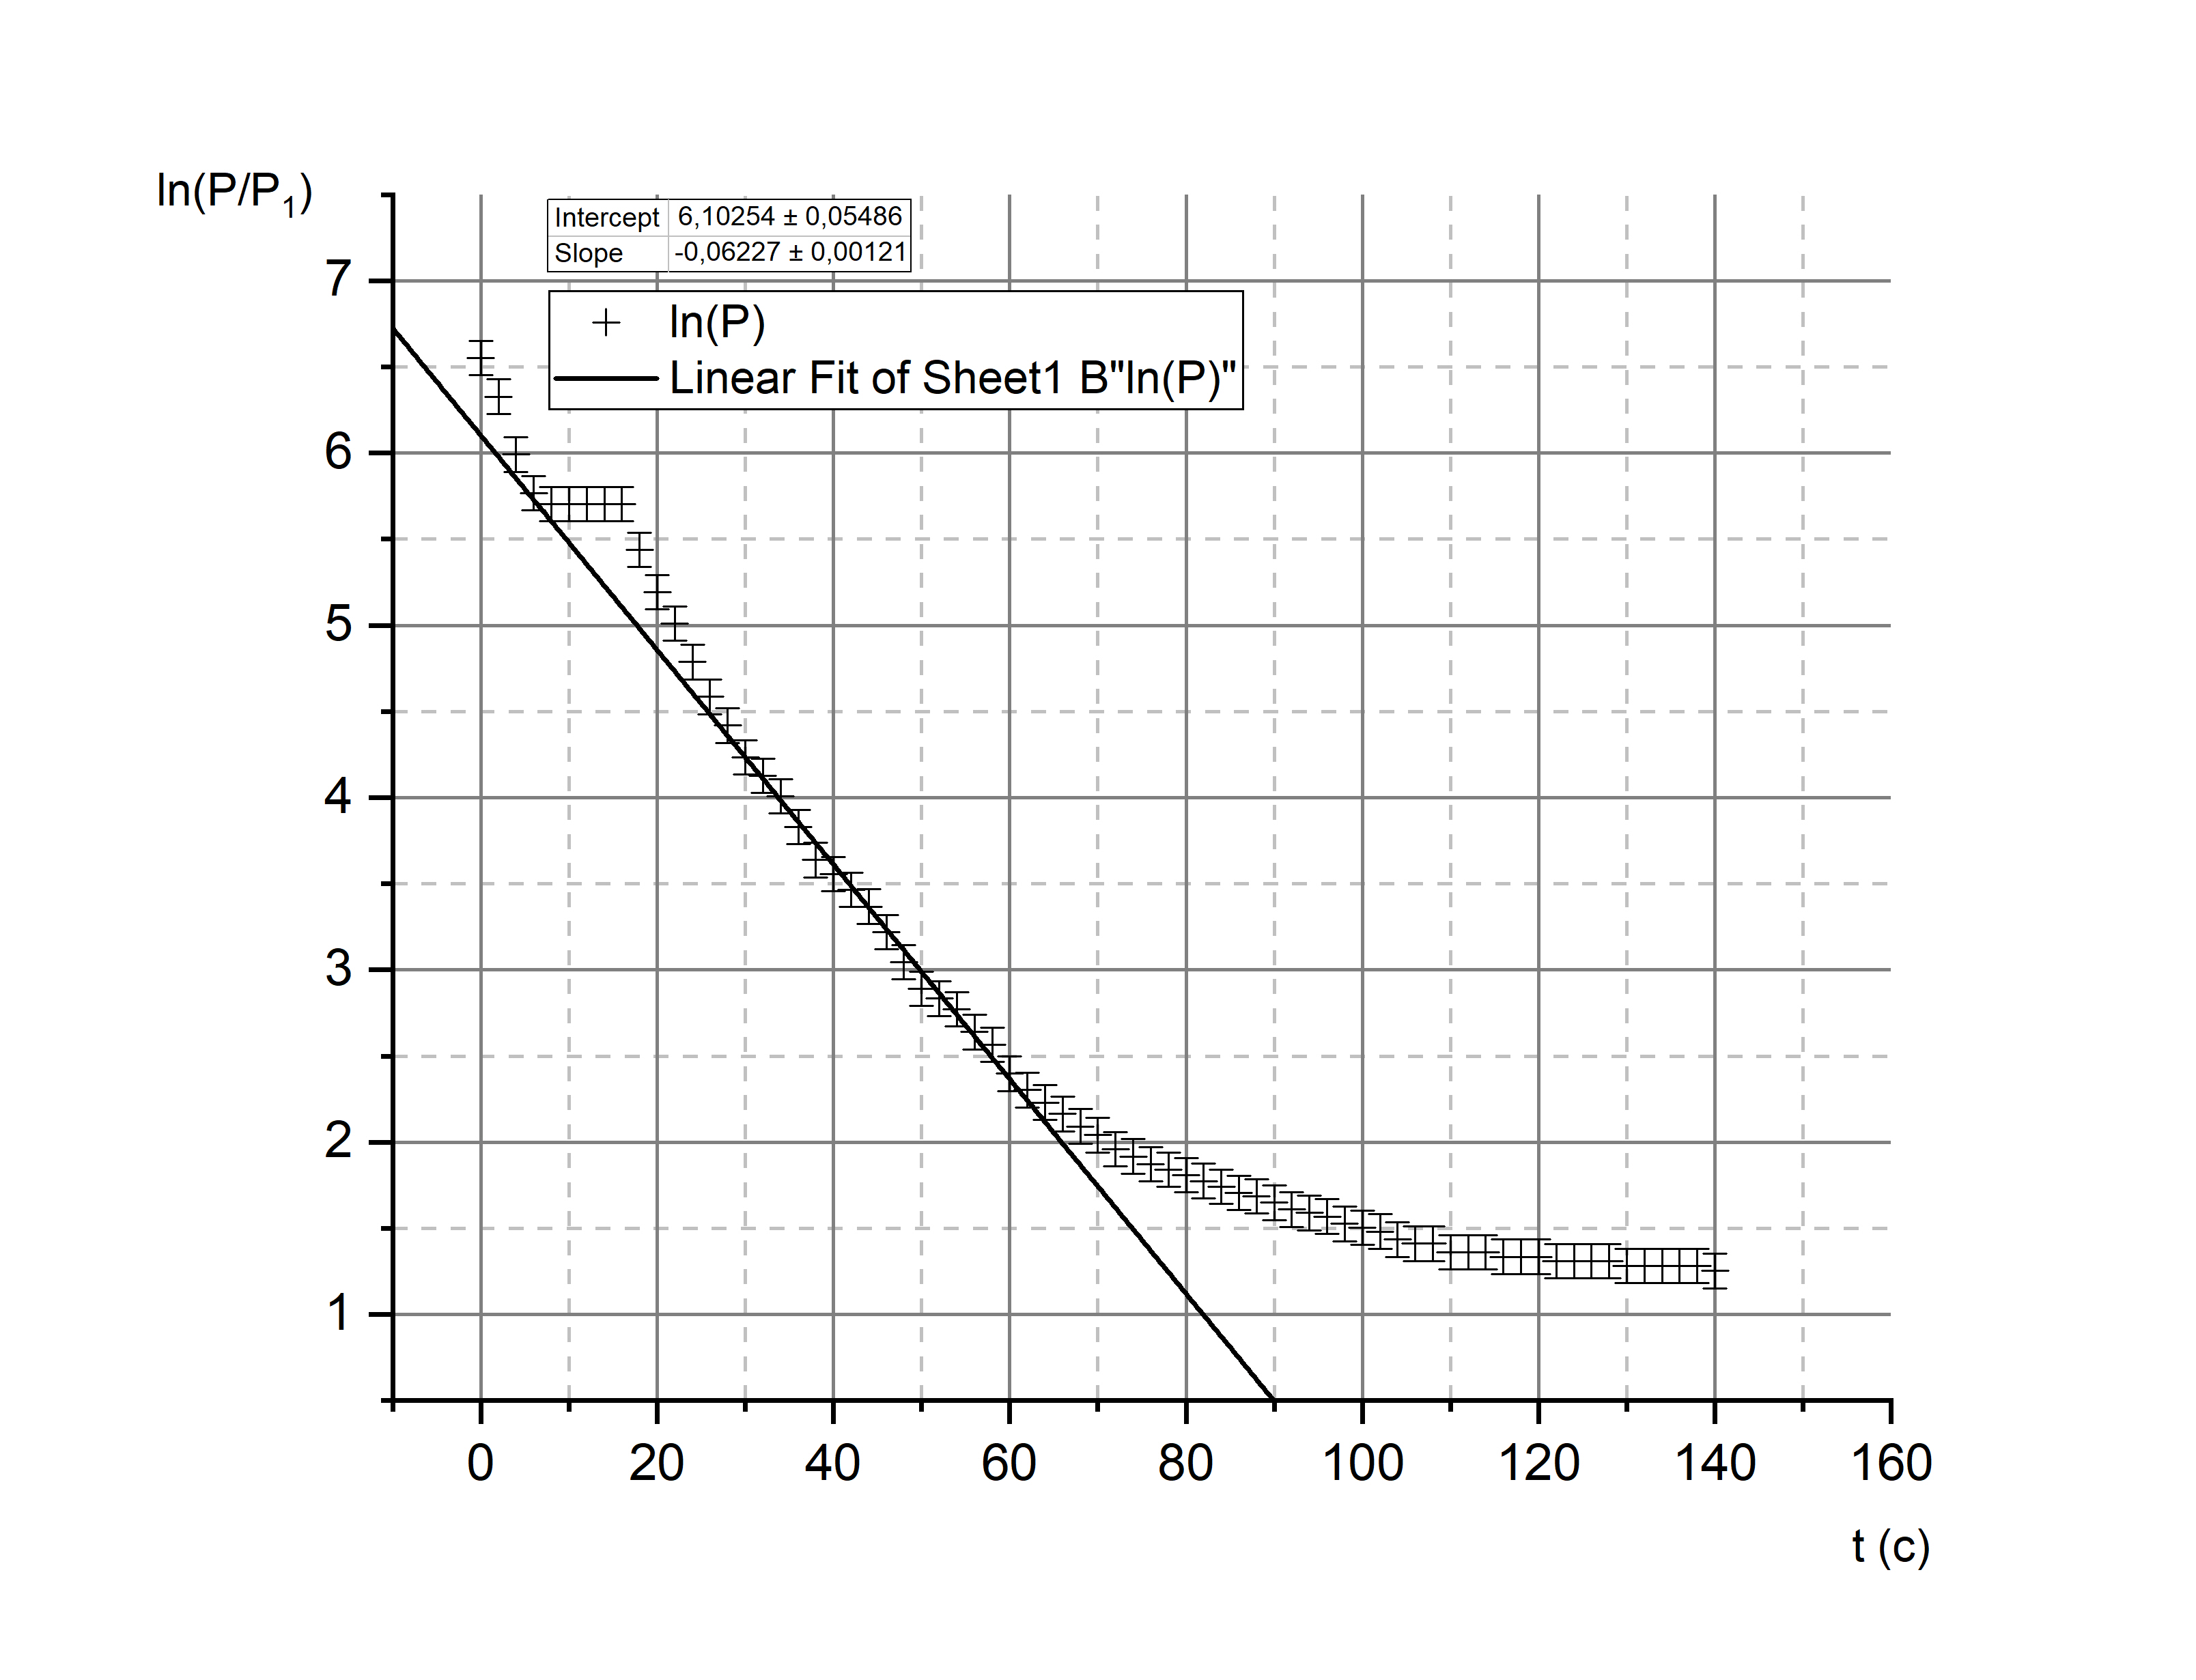
\includegraphics[width = \textwidth]{231_4.jpg}
\caption{График зависимости $ln(P/P_1)$ от $t$ для форвакуумного насоса}
\end{figure}
\end{enumerate}

\subsection*{Измерение скорости откачки турбомолекулярным насосом и определение предельного вакуума}
\begin{enumerate}
\item Откачиваем установку форвакуумным насосом.
\item Откачиваем объем турбомолекулярным насосом.
\item считаем скорость откачки воздуха $\tau \approx 0,049 c$, $S_0 \approx 49 l/c$

\begin{tabular}{|c|c|}
\hline
$t, c$ & $P, mbar$ \\ \hline
2 & 2,800000 \\ \hline
4 & 1,800000 \\ \hline
6 & 0,630000 \\ \hline
8 & 0,015000 \\ \hline
10 & 0,003800 \\ \hline
12 & 0,002400 \\ \hline
14 & 0,001500 \\ \hline
16 & 0,001100 \\ \hline
18 & 0,001000 \\ \hline
20 & 0,001000 \\ \hline
22 & 0,001000 \\ \hline
24 & 0,000870 \\ \hline
26 & 0,000660 \\ \hline
28 & 0,000580 \\ \hline
30 & 0,000500 \\ \hline
32 & 0,000390 \\ \hline
34 & 0,000350 \\ \hline
36 & 0,000310 \\ \hline
38 & 0,000280 \\ \hline
40 & 0,000240 \\ \hline
42 & 0,000190 \\ \hline
44 & 0,000180 \\ \hline
46 & 0,000170 \\ \hline
48 & 0,000150 \\ \hline
50 & 0,000140 \\ \hline
52 & 0,000130 \\ \hline
\end{tabular}
\begin{tabular}{|c|c|}
\hline
$t, c$ & $P, mbar$ \\ \hline
54 & 0,000120 \\ \hline
56 & 0,000110 \\ \hline
58 & 0,000100 \\ \hline
60 & 0,000095 \\ \hline
62 & 0,000091 \\ \hline
64 & 0,000088 \\ \hline
66 & 0,000083 \\ \hline
68 & 0,000080 \\ \hline
70 & 0,000076 \\ \hline
72 & 0,000073 \\ \hline
74 & 0,000069 \\ \hline
76 & 0,000067 \\ \hline
78 & 0,000065 \\ \hline
80 & 0,000064 \\ \hline
82 & 0,000062 \\ \hline
84 & 0,000061 \\ \hline
86 & 0,000059 \\ \hline
88 & 0,000058 \\ \hline
90 & 0,000057 \\ \hline
92 & 0,000055 \\ \hline
94 & 0,000054 \\ \hline
96 & 0,000053 \\ \hline
98 & 0,000052 \\ \hline
100 & 0,000051 \\ \hline
102 & 0,000050 \\ \hline
\end{tabular}
\begin{figure}[h]
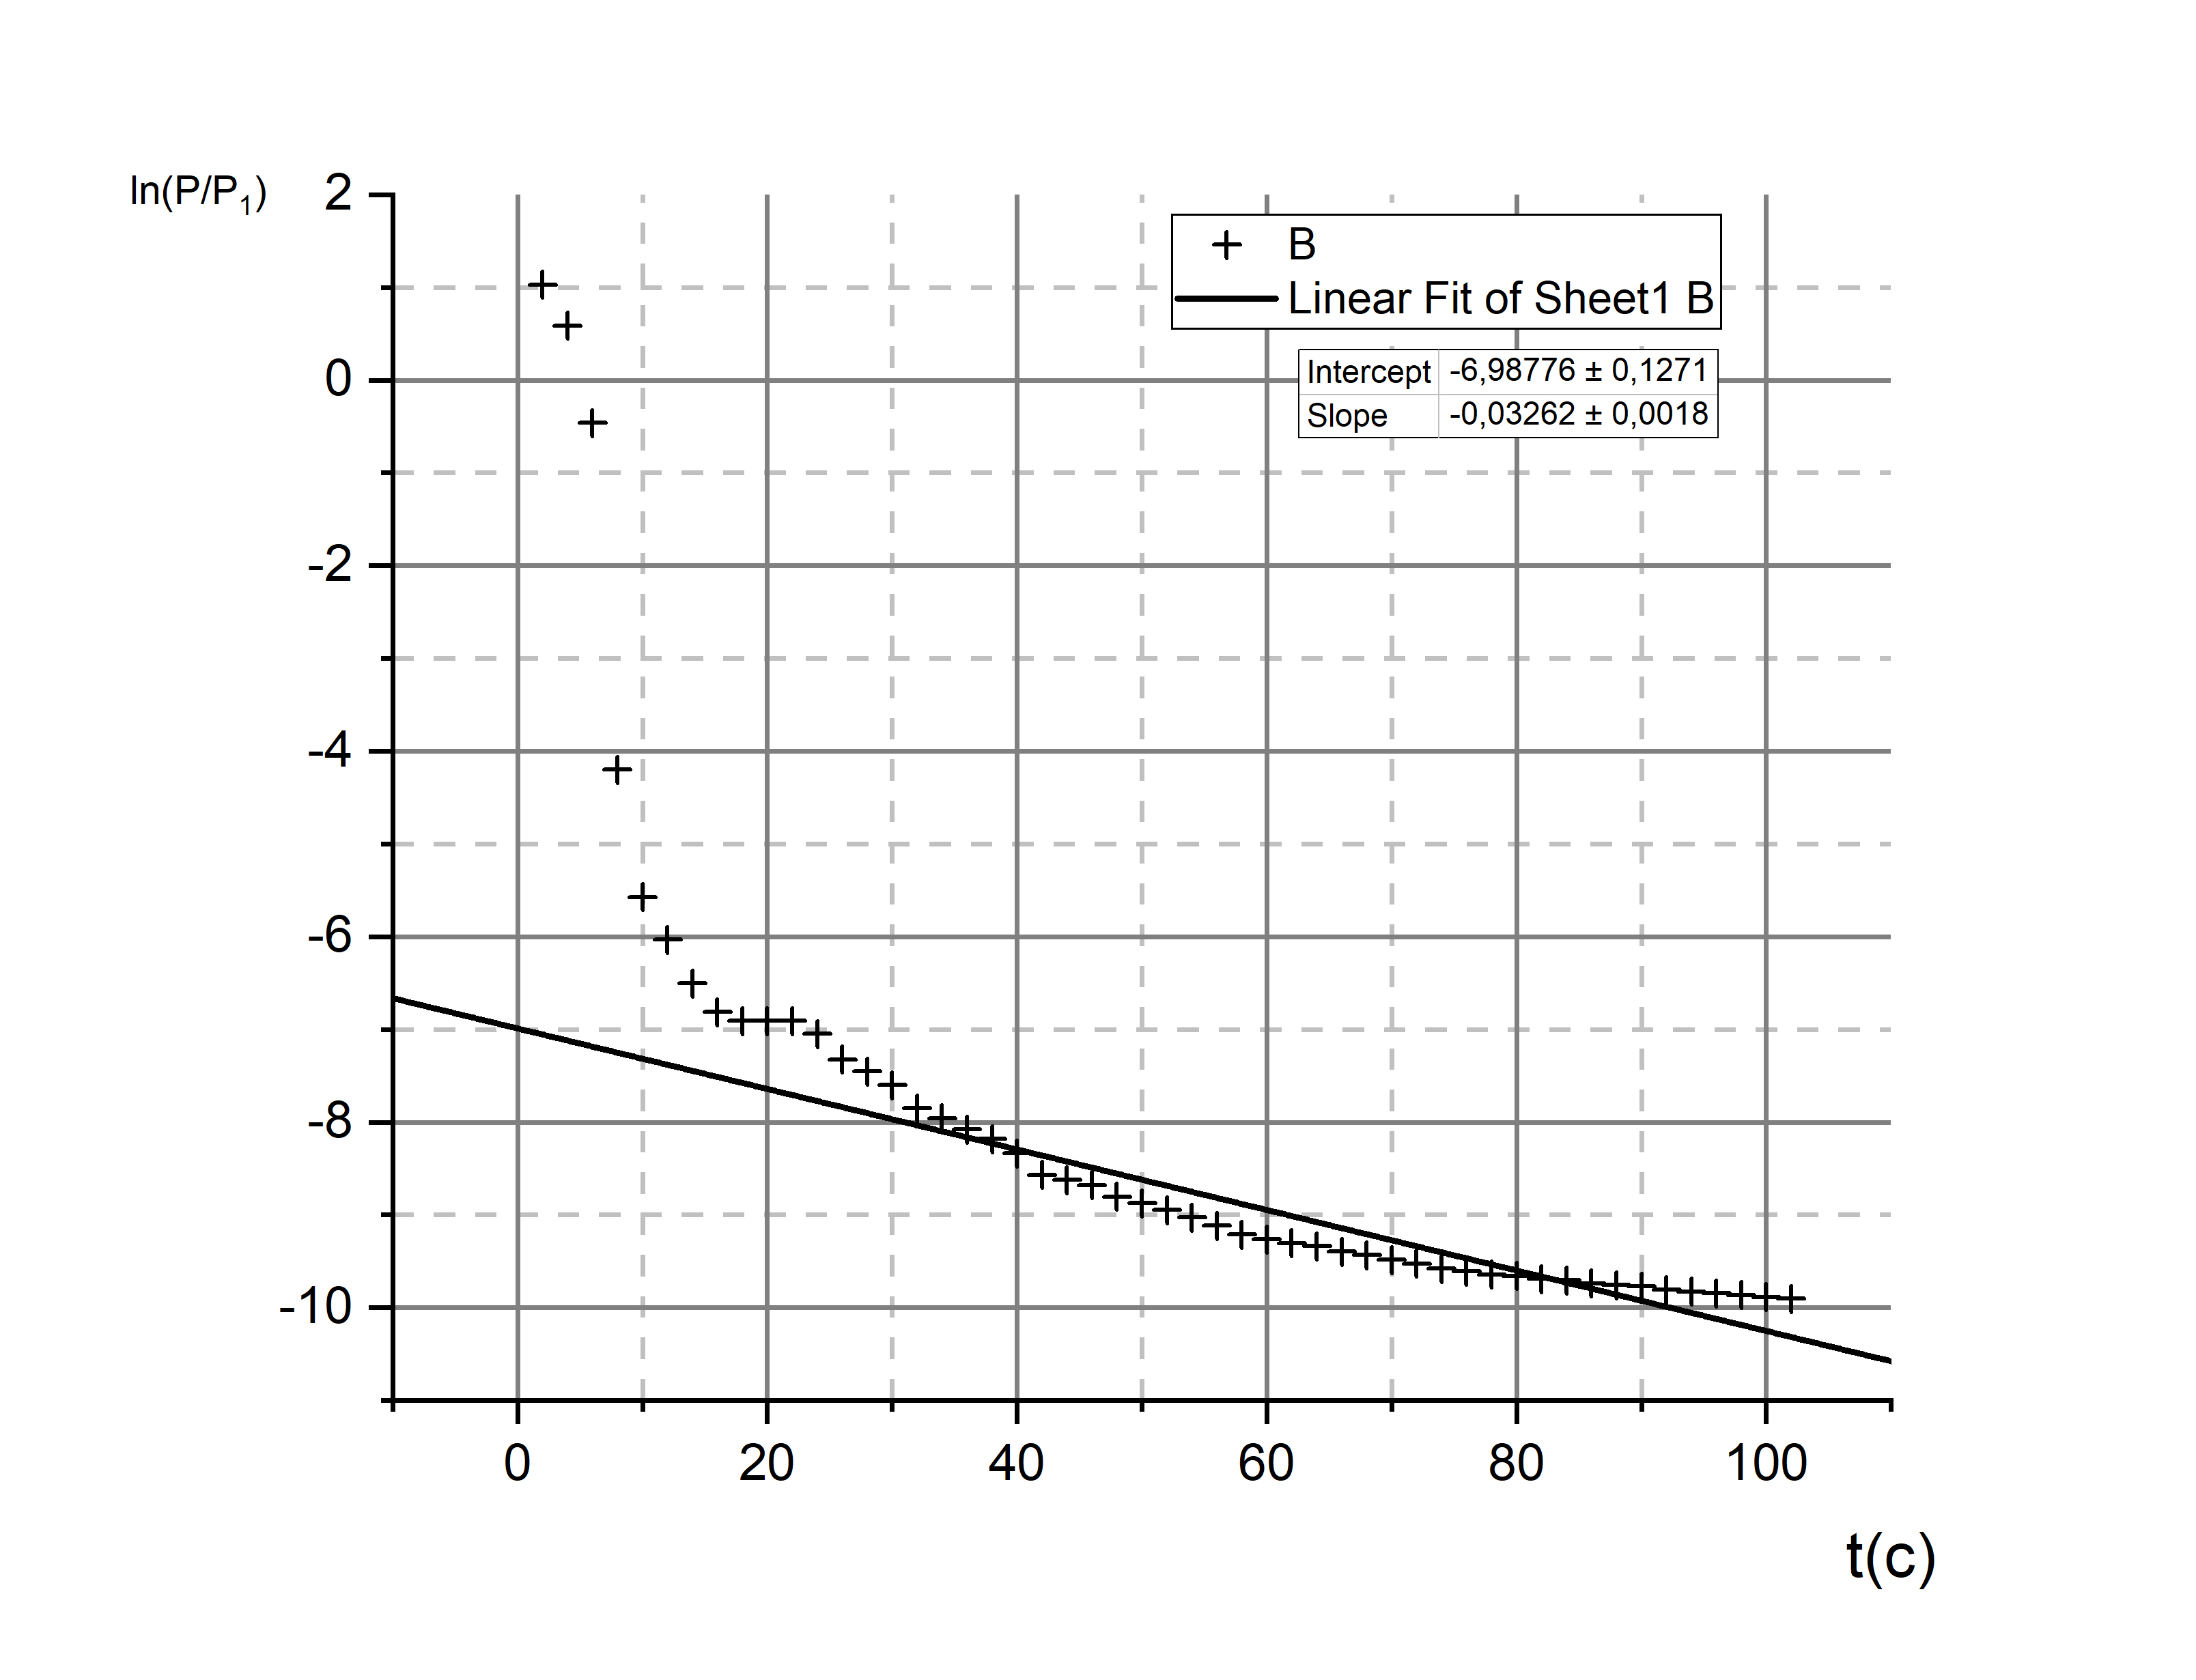
\includegraphics[width = \textwidth]{231_5.jpg}
\caption{График зависимости $ln(P/P_1)$ от $t$ для турбомолекулярного насоса}
\end{figure}
\item Определяем уровень течей по ухудшению вакуума после перекрытия насосом ТМН. Считаем $Q_{\text{н}} = V\dfrac{dP}{dt} \approx 1,4 l/c$
Проверяем, что выполяняется условие того, что $Q_{\text{н}} << Q$
\end{enumerate}
\end{document}